\section{Introduction}
In model-driven software engineering, the intensive use of generative programming techniques has become a common practice for software development since it reduces the development and maintenance effort by developing at a higher-level of abstraction through the use of domain-specific languages~\cite{brambilla2012model} (DSLs). 
DSLs, as opposed to general-purpose languages, are software languages that focus on specific problem domains. Thus, the realization of model-driven software development for a specific domain requires the creation of effective code generators and compilers for these DSLs.
Code-generation environments automate and systematize the process of building families of software systems which can clearly reduce the effort of software implementation.
%The use of code generators is needed to transform manually designed models to software artifacts, which can be deployed on different target platforms. 
Indeed, a code generator is needed to transform manually designed models (source code programs represented in a graphical/textual modeling language) to general purpose programming languages such as C, Java, C++, etc. In turn, generated code is transformed into machine code (binaries) using a set of specific compilers.
These compilers serve as a basis to target different ranges of platforms. 
%Many technologies, such as Docker containers, provide new opportunities to automate the deployment of produced code into a distributed and heterogeneous component-based infrastructure
However, code generators can be difficult to understand since they involve a set of complex and heterogeneous technologies which make the task of performing design, implementation, and testing very hard and time-consuming[ref]. Code generators have to respect different requirements which preserve software reliability and quality. In fact, a defective code generator can generate defective software artifacts which range from uncompilable or semantically dysfunctional code that causes serious damage to the target platform, to non-functional bugs which lead to poor-quality code that can affect system reliability and performance (e.g., high resource usage, execution speed, etc.). 
%Thus, these issues should be corrected by hand each time the code generator triggers functional or non-functional failures.

Generally, in order to check the correctness of code generation process, developers often use to define (at design time) a set of test cases that verify the functional outcome of generated code. Afterwards, test cases are executed within each target platform which can lead to either a correct behavior or a failure (e.g., crashes, bugs). 
For non-functional testing of code generators, developers need to deploy and execute software artifacts within different execution platforms. Then, they have to collect and visualize information about the performance and efficiency of generated code. Finally, they report issues related to the code generation process such as incorrect typing, memory management leaks. etc. To do so, developers generally use several platform-specific profilers, trackers, and monitoring tools in order to find some inconsistencies or bugs during code execution. Ensuring the code quality of generated code can refer to several non-functional properties such as code size, resource or energy consumption, execution time, among others [ref]. Therefore, we believe that testing the non-functional properties of code generators remains challenging and time-consuming task because developers have to analyze and verify code for each target platform using platform-dependent tools.

This paper describes a runtime monitoring infrastructure based on system containers, as execution platform, to evaluate the consistency and coherence of generated code regarding the non-functional properties. This approach provides a fine-grained understanding of resource consumption and analysis of components behavior. 
We evaluate our approach by analyzing the non-functional properties of HAXE, a popular high-level language that involves a set of cross-platform code generators able to compile to different targets. Our initial experimental results show that our approach is able to detect non-functional bugs within HAXE code generators.

\begin{figure*}[h]
	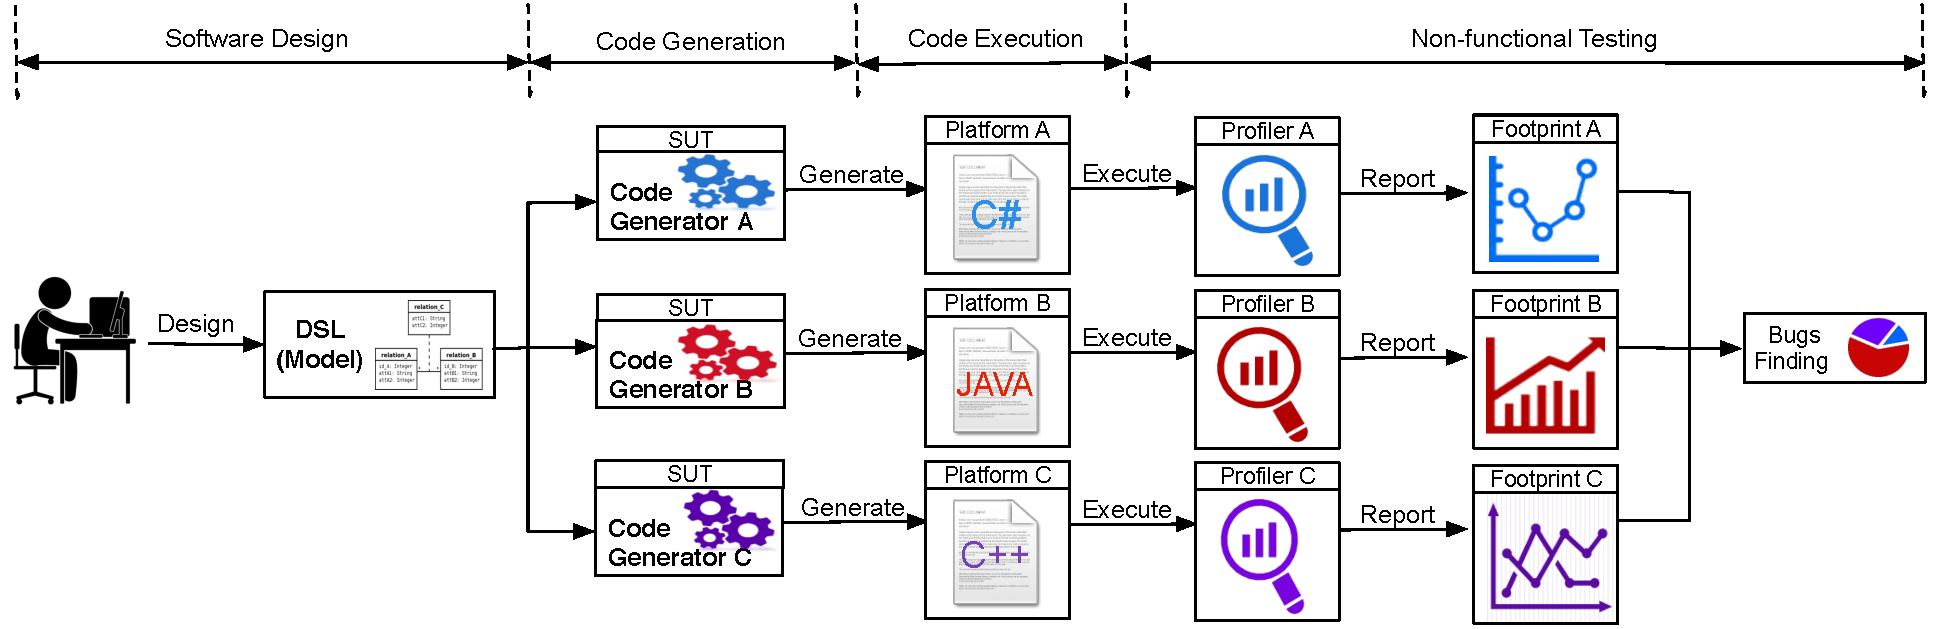
\includegraphics[width=1\linewidth]{Ressources/background.pdf}
	\caption{An overall overview of the different processes involved to ensure the code generation and non-functional testing of produced code from design time to runtime.}
	%		\label{AAA}
\end{figure*}

%In fact, during the code generation process, different optimizations may be applied for code transformation. Improvement of source program can refer to several different characteristics of the produced code such execution time, memory consumption, code size, among others~\cite{almagor2004finding,pan2006fast}.
%For example, embedded systems for which code is generated often have limited resources. 
%\begin{figure}[h]
%	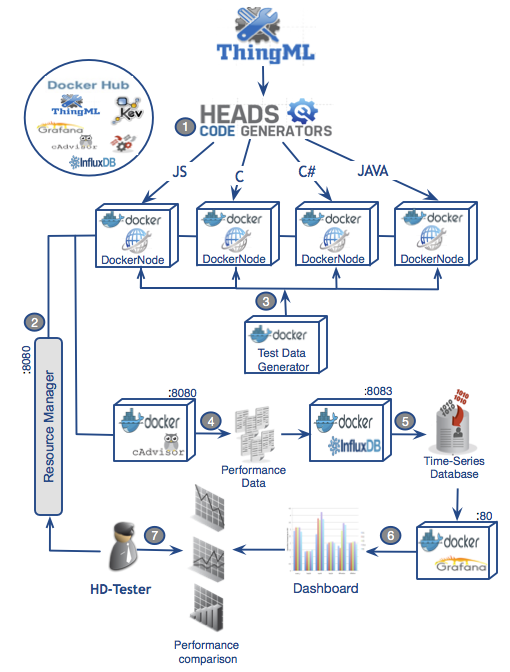
\includegraphics[width=1.\linewidth]{Ressources/app.png}
%	\caption{Overview of the Docker-based testing architecture}
%\end{figure}




%Model-based code generators integrate rule-based model-to-model transformation languages such as ATL and template-based model-to-text transformation languages such as Acceleo to translate high-level system specifications into executable code and scripts. A








%\cleardoublepage
%Therefore, optimization techniques must be applied whenever possible to generate efficient code with respect to available resources\cite{nagiub2013automatic}. 
%As general-purpose optimizations, compiler creators\footnote{We consider compilers as a kind of code generators in this paper. Indeed, from the testing point of view, we do not make any differences between testing code generators and testing compilers} usually define fixed and program-independent sequence optimizations.
%For example, in GCC, we can distinguish optimization levels from O1 to O3. Each optimization level involves a fixed list of compiler optimization options. 
%However, industrial code generators may have a huge number of potential optimization combinations, making it hard and time-consuming for software developers to find the sequence of optimizations that satisfies user key objectives. 

%In this paper we explore the relationship between runtime execution of optimized code and non-functional properties.
%We propose a component-based tooled approach to check code generators non-functional properties through the monitoring of generated code in a controlled sandboxing environment. 
%Our approach is based on microservices to automate the deployment and monitoring of different variants of optimized code into a distributed and heterogeneous component-based infrastructure. 
%We assess the effectiveness of our approach by evaluating the optimizations performed by the GCC compiler, a widely used compiler in software engineering community. 
%We also present a number of case studies, in which the tool was successfully used.
%This to ensure the efficiency of generated code, deployed components must be checked and verified regarding their non-functional behavior
%\footnote{\url{https://www.docker.com}} 

%The primary contribution of this paper can be summarized as follows: 
%(1) We propose a microservice infrastructure to ensure the deployment and monitoring of generated code regarding resource consumption; 
%(2) We evaluate the effectiveness of our approach by testing the GCC compiler optimizations across two case studies.
 

The paper is organized as follows.
Section II describes the motivation behind this work. We present in Section III our infrastructure for non-functional testing using microservices. 
The evaluation and results of our experiments are discussed in Section IV. 
Finally, related work, concluding remarks and future work are provided in Sections V and VI.


%The difference between classical compilers like GCC, LLVM and code generators is that code generators are used only by few people comparing to famous compilers like GCC. Moreover, code generators face a high rate of changes and update versions due to new development needs. Hence, it becomes necessary to check the quality of produced code. This will help software maintainers to verify the correct functioning of code generators.  Among the most important properties to check, we distinguish the non functional properties.

%Like traditional compilers, code generators typically perform multiple passes over various intermediate forms during code transformation. Many rules may also be applied and that differs from one generator to another. These passes are complex and highly dependent on target platform architecture. 

 
 

  % \section{Motivations}
 %\section{Previous work}
%\section{Approach Overview}
